\documentclass[11pt]{article}
\usepackage[margin=1in, top=1in]{geometry}
\usepackage[all]{nowidow}
\usepackage[hyperfigures=true, hidelinks, pdfhighlight=/N]{hyperref}
\usepackage[separate-uncertainty=true, group-digits=false]{siunitx}
\usepackage{graphicx,amsmath,physics,tabto,float,amssymb,pgfplots,verbatim,tcolorbox}
\usepackage{listings,xcolor,subfig,caption,import,wrapfig,pdfpages}
\usepackage[version=4]{mhchem}
\usepackage[noabbrev]{cleveref}
\newcommand{\creflastconjunction}{, and\nobreakspace}
\numberwithin{equation}{section}
\numberwithin{figure}{section}
\numberwithin{table}{section}
\definecolor{stringcolor}{HTML}{C792EA}
\definecolor{codeblue}{HTML}{2162DB}
\definecolor{commentcolor}{HTML}{4A6E46}
\captionsetup{font=small, belowskip=0pt}
\lstdefinestyle{appendix}{
    basicstyle=\ttfamily\footnotesize,commentstyle=\color{commentcolor},keywordstyle=\color{codeblue},
    stringstyle=\color{stringcolor},showstringspaces=false,numbers=left,upquote=true,captionpos=t,
    abovecaptionskip=12pt,belowcaptionskip=12pt,language=Python,breaklines=true,frame=single}
\lstdefinestyle{inline}{
    basicstyle=\ttfamily\footnotesize,commentstyle=\color{commentcolor},keywordstyle=\color{codeblue},
    stringstyle=\color{stringcolor},showstringspaces=false,numbers=left,upquote=true,frame=tb,
    captionpos=b,language=Python}
\renewcommand{\lstlistingname}{Appendix}
\pgfplotsset{compat=1.17}

\begin{document}

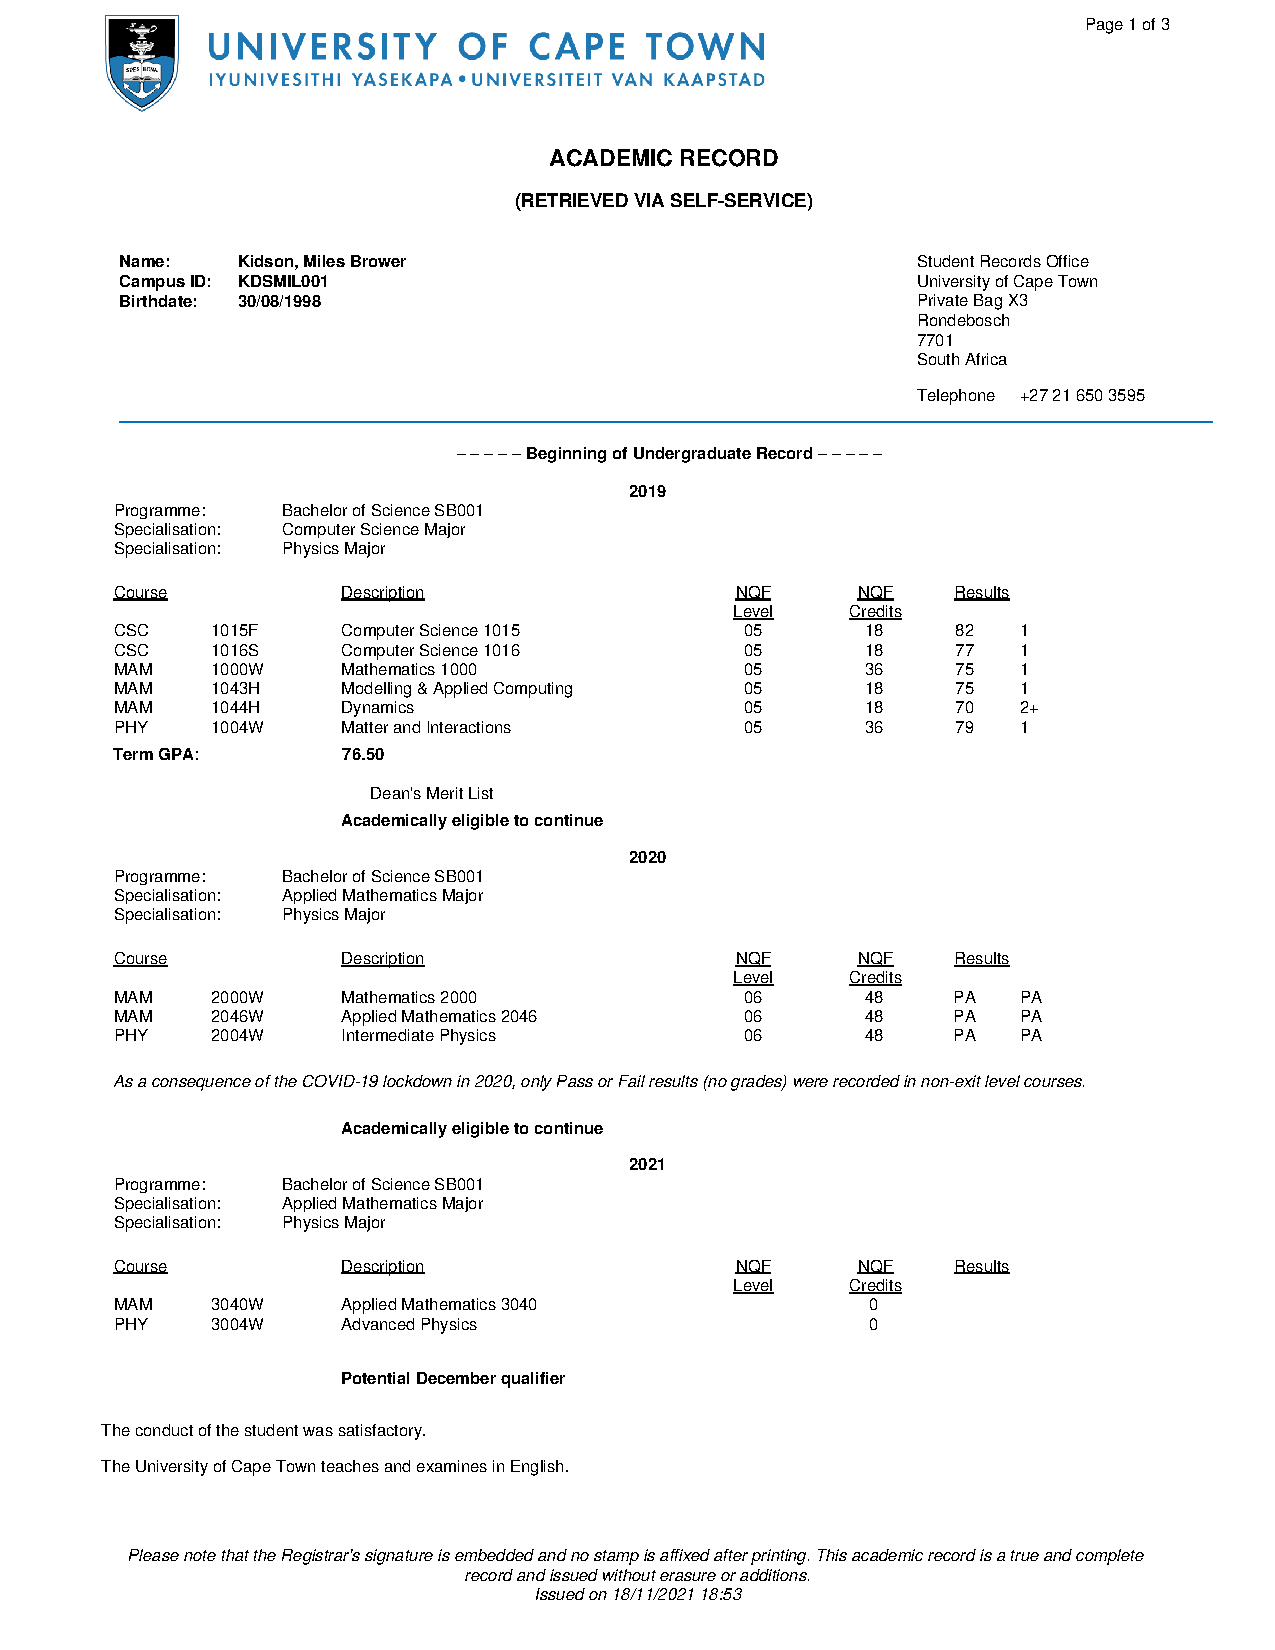
\includepdf[pages=-]{UCT_SRETSRPT.pdf}

\section*{Motivation}
Currently my interest is in Nuclear Physics. My third year project concerned digital pulse shape discrimination to discriminate between neutron and photon events in an EJ301 liquid scintillator detector. Neutrons are a particularly interesting topic to me as they don’t interact as much as charged particles, for example. This makes studying them quite tricky, hence the third year project topic. I also have interests in Particle Physics. The standard model is the best guess we have to describe the fundamental particles but clearly there is more to be discovered and as our experimental techniques improve, so will our theories. I am definitely more interested in the experimental side of things rather than the theoretical, and I think I am quite suited to computational tasks, so I’m hoping to head towards that direction, perhaps with the ALICE or ATLAS collaborations.
\end{document}